\chapter{REFERENCIAL TEÓRICO}
\label{chap:referencialTeorico}

Este capítulo apresenta a revisão bibliográfica dos conceitos fundamentais que sustentam o problema de pesquisa e a arquitetura proposta nesta dissertação, abrangendo Redes Definidas por Software, programabilidade do plano de dados com P4 e eBPF/XDP, protocolos de roteamento na origem com ênfase no PolKA, Redes Cientes de Caminho, fatiamento de redes (\textit{Network Slicing}), mecanismos de Qualidade de Serviço e escalonamento programável, controle de congestionamento e a análise dos trabalhos relacionados.

% ==============================================================================
\section{Redes Definidas por Software e Planos de Dados Programáveis}
\label{sec:sdn_programabilidade}

\subsection{Conceitos Gerais de SDN}
\label{subsec:conceitos_sdn}

No âmbito das redes de computadores, a Engenharia de Tráfego (\textit{Traffic Engineering} -- TE) compreende o conjunto de técnicas voltadas à medição, modelagem e controle dos fluxos de dados, visando assegurar a eficiência operacional da infraestrutura de comunicação. Seu objetivo primordial consiste em maximizar o aproveitamento da largura de banda e prevenir cenários de congestionamento, viabilizando o cumprimento de parâmetros estritos de Qualidade de Serviço (\textit{Quality of Service} -- QoS) por meio do tratamento prioritário de aplicações sensíveis ou de missão crítica.

Para que a TE atue de forma preditiva e adaptativa --- identificando padrões de tráfego, sazonalidades ou anomalias ---, as redes demandam flexibilidade e mecanismos dinâmicos de reconfiguração em tempo real. Nesse cenário, as arquiteturas convencionais enfrentam entraves devido ao acoplamento entre a tomada de decisão e o encaminhamento físico. Essa limitação impulsionou o surgimento das Redes Definidas por Software (\textit{Software-Defined Networking} -- SDN), paradigma que introduz a separação explícita entre o plano de controle (responsável pela inteligência e pelas decisões de roteamento) e o plano de dados (encarregado unicamente do trânsito e da comutação dos pacotes). Essa separação é ilustrada pela Figura~\ref{fig:arquitetura_sdn}.

\begin{figure}[!htbp]
    \centering
    \caption{Arquitetura SDN.}
    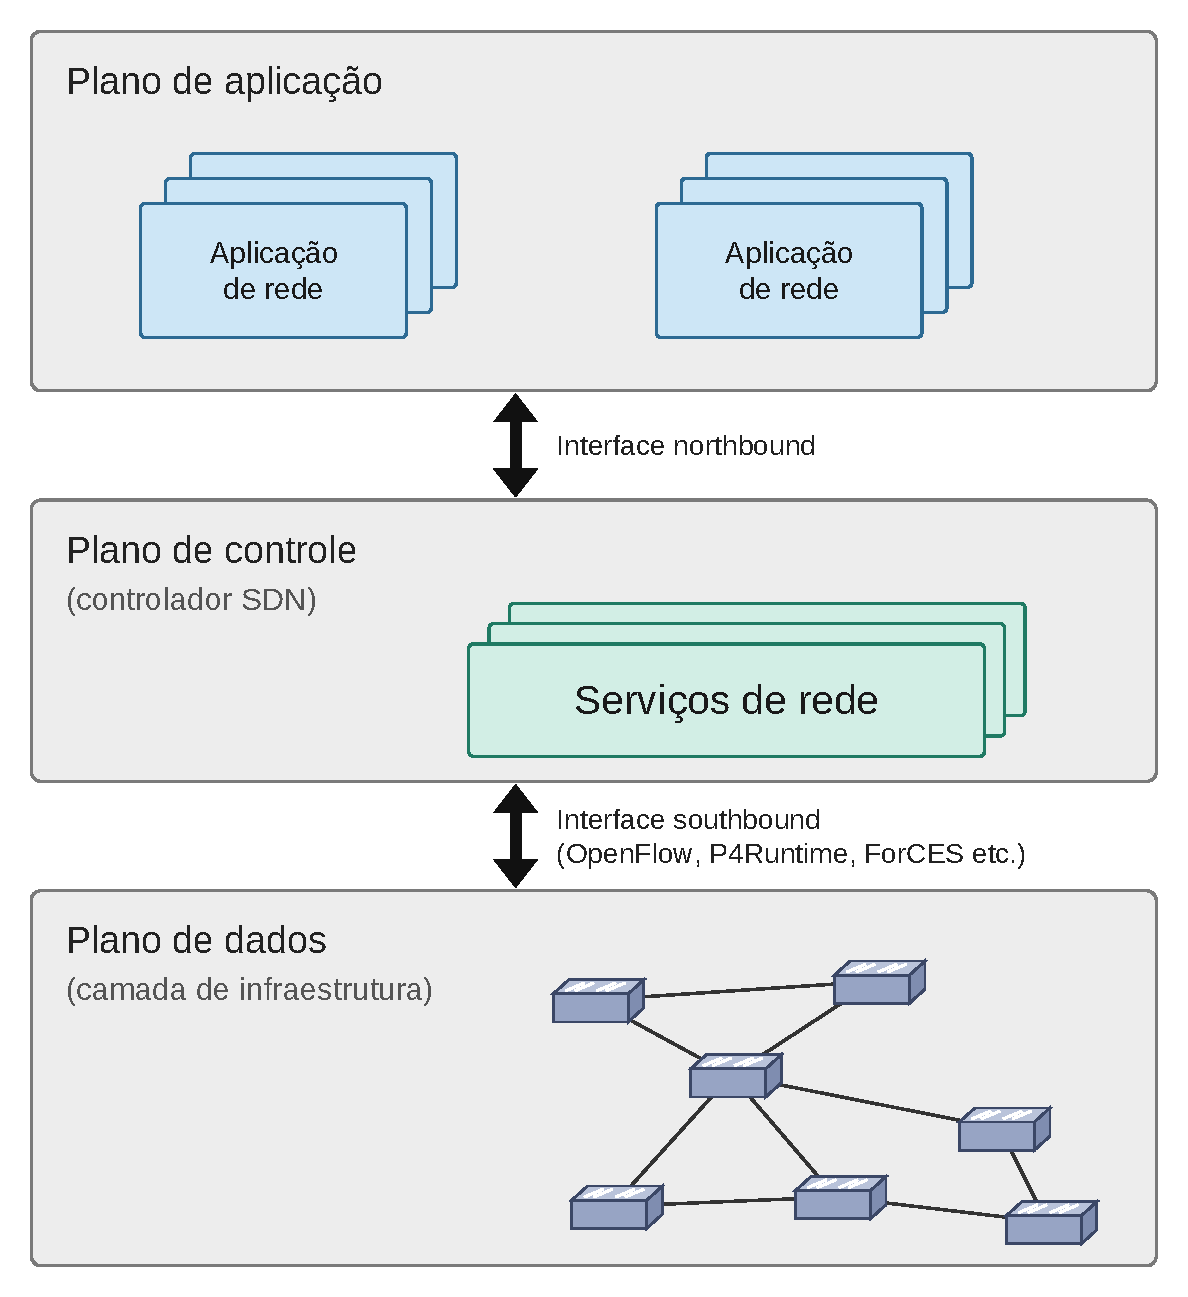
\includegraphics[width=0.6\textwidth]{figuras/arquitetura_sdn.pdf}
    \label{fig:arquitetura_sdn}
    \fonte{Adaptado de \textcite{katukam2013sdn}.}
\end{figure}

Ao centralizar logicamente o plano de controle em uma entidade denominada controlador SDN, a rede ganha visibilidade global e capacidade de abstração do hardware subjacente. Em contraposição aos modelos tradicionais, nos quais os dispositivos operam com inteligência distribuída e tabelas configuradas individualmente de forma autônoma ou estática, a abordagem SDN permite gerenciar políticas de segurança, balanceamento e alocação de largura de banda de maneira coordenada e automatizada a partir de um único núcleo de controle.

\subsection{Linguagem P4}
\label{subsec:linguagem_p4}

Os dispositivos de rede apresentam diferentes níveis de programabilidade consoante a sua arquitetura de concepção. Tradicionalmente, grande parte dos equipamentos em operação possui um plano de dados estático e fechado, o que restringe severamente a incorporação de novos protocolos e dificulta a avaliação empírica de propostas de encaminhamento não padronizadas pelos fabricantes.

A linguagem P4 (\textit{Programming Protocol-independent Packet Processors}) surge como uma linguagem de domínio específico concebida precisamente para especificar e programar a lógica de funcionamento do plano de dados em elementos de encaminhamento, como comutadores (\textit{switches}) e roteadores. Distinguindo-se da abordagem introduzida pelo OpenFlow --- que se apoiava em tabelas de fluxo com cabeçalhos e correspondências pré-definidas ---, o P4 outorga ao desenvolvedor a capacidade de determinar como os pacotes de rede devem ser descompactados (\textit{parsing}), analisados, modificados e reencaminhados de maneira totalmente independente de protocolos pré-estabelecidos. Torna-se, assim, viável a criação ou adaptação de formatos de cabeçalhos, a customização de primitivas de processamento e a especificação detalhada de cada etapa do \textit{pipeline} de comutação \cite{KAUR2021109}.

\begin{figure}[!htbp]
    \centering
    \caption{Fluxo de trabalho de um programa P4.}
    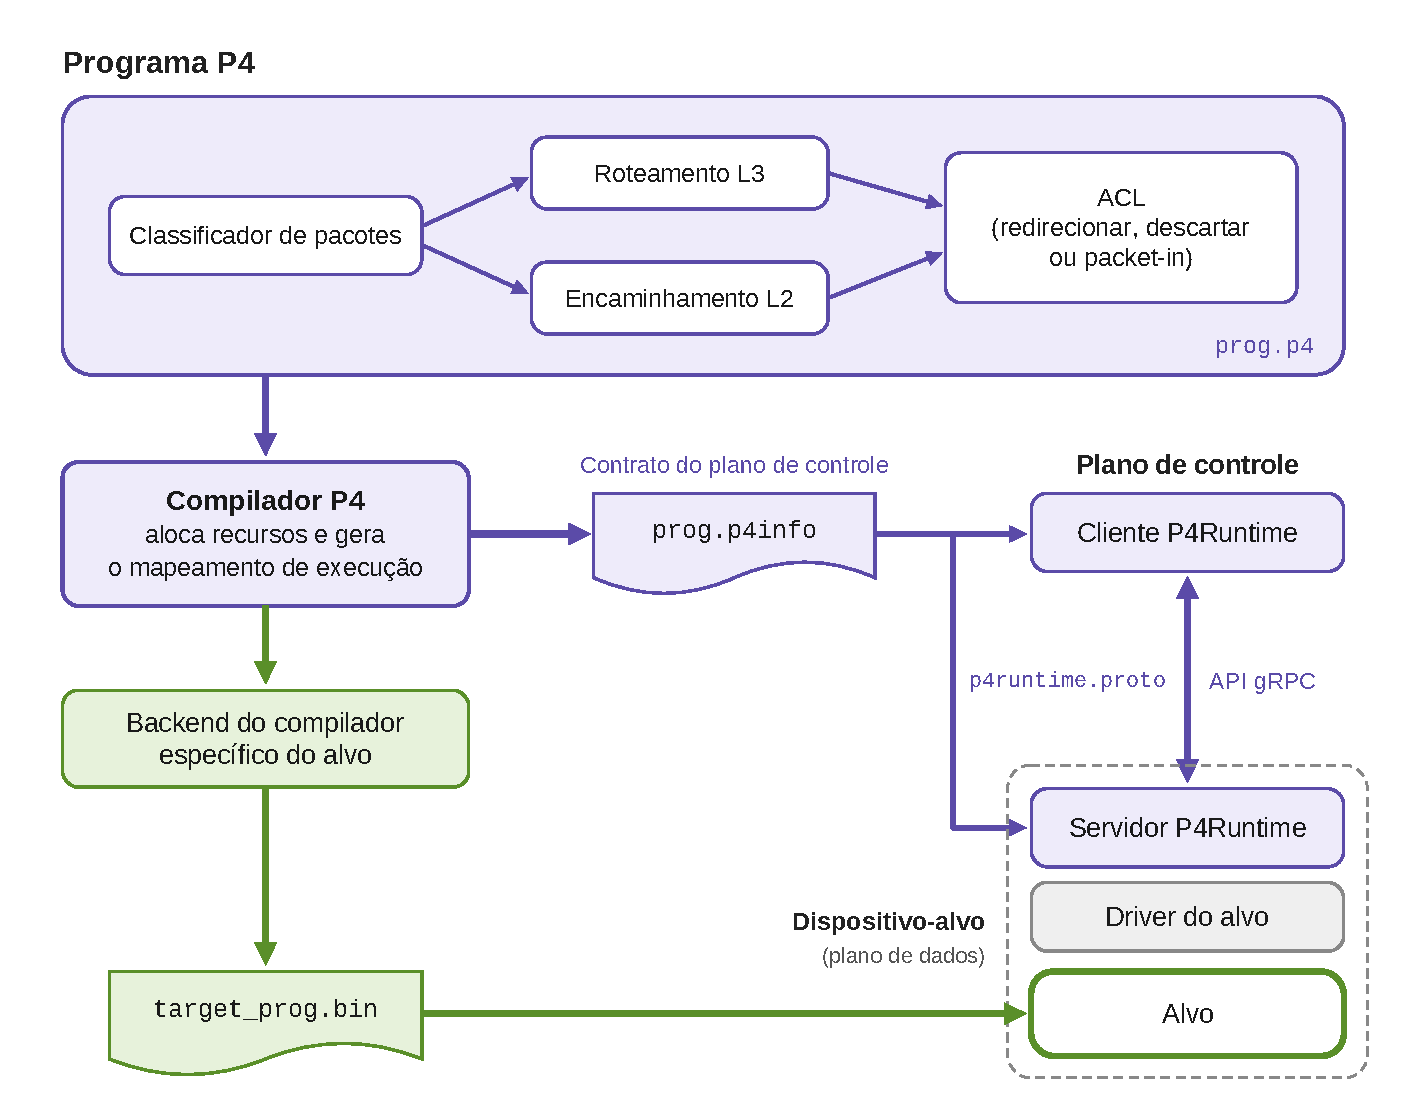
\includegraphics[width=0.85\textwidth]{figuras/fluxo_p4.pdf}
    \label{fig:fluxo-p4}
    \fonte{Adaptado de \textcite{p4org2025workflow}.}
\end{figure}

A Figura~\ref{fig:fluxo-p4} ilustra o fluxo de trabalho típico da programação de um dispositivo P4. Para cada alvo (\textit{target}), o fabricante fornece um modelo de arquitetura, que define os blocos programáveis e as interfaces disponíveis, e um compilador P4 específico. O compilador mapeia o programa P4 para os recursos desse alvo e gera dois artefatos: a configuração do plano de dados (\texttt{target\_prog.bin}), que implementa a lógica de processamento de pacotes descrita no programa, e o arquivo \texttt{P4Info} (\texttt{prog.p4info}), que atua como contrato entre os planos de controle e de dados, descrevendo as tabelas, ações e demais objetos gerenciados em tempo de execução por meio da API \textit{P4Runtime}.

Essa capacidade de parametrizar o processamento dos fluxos diretamente no circuito de encaminhamento constitui um marco na evolução das Redes Definidas por Software. Por intermédio do P4, projetistas e pesquisadores adquirem autonomia para conceber, homologar e implementar arquiteturas de encaminhamento e mecanismos de otimização de tráfego, prescindindo dos longos ciclos de atualização de \textit{firmware} fechado ou da substituição de plataformas proprietárias.

\subsection{Tecnologia eBPF e XDP}
\label{subsec:tecnologia_ebpf}

O \textit{Extended Berkeley Packet Filter} (eBPF) consiste em uma tecnologia de infraestrutura que atua como uma máquina virtual leve de 64~bits integrada ao núcleo (\textit{kernel}) do Linux, projetada para executar código customizado, seguro e de alto desempenho em tempo de execução sem requerer modificações no código-fonte nem a inclusão de módulos proprietários no sistema operacional \cite{sharaf2022extended}. Trata-se de uma evolução substancial da arquitetura clássica \textit{Berkeley Packet Filter} (cBPF) --- originalmente voltada apenas para a captura estática de pacotes e filtragem de chamadas de sistema ---, ampliando seu alcance para uma plataforma programável genérica e orientada a eventos, cujas instruções são compiladas dinamicamente em código de máquina nativo via JIT (\textit{Just-In-Time}) e submetidas a um rigoroso verificador estático (\textit{verifier}) in-kernel que assegura a terminação do programa e a segurança dos acessos à memória \cite{di2019berkeley}.

No âmbito do processamento de tráfego de rede e da implementação de Funções de Rede Virtualizadas (\textit{Network Functions Virtualization} -- NFV), o eBPF viabiliza a criação de planos de dados de alto rendimento ancorados diretamente aos pontos de acoplamento (\textit{hooks}) do subsistema de rede do Linux \cite{sharaf2022extended}, destacando-se dois níveis principais de atuação:
\begin{itemize}
    \item \textbf{\textit{eXpress Data Path} (XDP):} intercepta os pacotes diretamente no \textit{driver} da placa de rede (NIC) logo após a recepção pelo anel de entrada (\textit{Rx ring}) e antes da alocação da estrutura de metadados de rede do \textit{kernel} (\texttt{struct sk\_buff}), reduzindo drasticamente a sobrecarga de CPU para ações imediatas de descarte (\texttt{XDP\_DROP}), redirecionamento (\texttt{XDP\_REDIRECT}) ou reescrita de cabeçalhos \cite{miano2018creating};
    \item \textbf{\textit{Traffic Control} (TC BPF):} opera nos ganchos de ingresso e egresso do subsistema de controle de tráfego do Linux sobre a estrutura \texttt{struct \_\_sk\_buff}, permitindo tanto a inserção de novos cabeçalhos de encapsulamento quanto a integração direta com disciplinas nativas de enfileiramento e modelagem de tráfego (\textit{qdiscs}) \cite{sharaf2022extended}.
\end{itemize}

Por fim, a retenção de estado e o compartilhamento bidirecional de dados entre as rotinas em execução no núcleo e os processos de gestão no espaço do usuário (\textit{user space}) estruturam-se sobre os \textit{eBPF Maps} \cite{sharaf2022extended}. Essas estruturas do tipo chave-valor --- tais como tabelas \textit{hash}, arranjos e árvores de correspondência de prefixo mais longo (\textit{LPM Trie}) --- podem ser fixadas no sistema de arquivos virtual BPF (\texttt{/sys/fs/bpf}), permitindo a atualização dinâmica de políticas de encaminhamento e a coleta não intrusiva de telemetria \cite{miano2018creating}.

% ==============================================================================
\section{Protocolos de Roteamento na Origem}
\label{sec:roteamento_origem}

Os protocolos de Roteamento na Origem (\textit{Source Routing} -- SR) constituem um paradigma no qual a determinação da trajetória percorrida pelos pacotes é transferida dos elementos intermediários da infraestrutura para o nó emissor ou comutador de borda. Sob esse modelo, o ponto de ingresso define explicitamente a sequência de saltos necessária para alcançar o destino, encapsulando essas instruções diretamente em um cabeçalho específico anexado ao pacote \cite{dominicini2020}.

Essa abordagem concede à origem controle minucioso sobre o trajeto dos fluxos, sendo particularmente vantajosa para a imposição de políticas estritas de engenharia de tráfego, execução de testes de desempenho e monitoramento de enlaces. Embora a necessidade de conhecimento prévio da topologia completa represente um desafio em arquiteturas distribuídas convencionais, o \textit{Source Routing} integra-se de forma sinérgica com as Redes Definidas por Software (SDN), nas quais a visibilidade global do controlador central permite calcular percursos ótimos e codificar as decisões de encaminhamento diretamente nos pacotes na borda da rede \cite{ventre2020segment}.

No âmbito operacional, os protocolos de SR dividem-se em duas abordagens principais:
\begin{itemize}
    \item \textbf{Roteamento Estrito na Origem (\textit{Strict Source Routing}):} o trajeto é determinado de forma exata e mandatória, especificando cada nó intermediário e interface de saída no cabeçalho; o pacote deve transitar estritamente pela sequência delimitada, sem desvios;
    \item \textbf{Roteamento Livre na Origem (\textit{Loose Source Routing}):} a origem define apenas pontos-chave ou nós de passagem obrigatórios ao longo do percurso, enquanto os segmentos intermediários entre esses pontos são resolvidos dinamicamente por protocolos de roteamento convencionais.
\end{itemize}

Arquiteturas modernas como o \textit{Segment Routing} (SR-MPLS e SRv6) \cite{rfc8402, ventre2020segment} e o \textit{Path Switching} \cite{hari2015pathswitching} mitigam a manutenção de estados por fluxo no núcleo da rede. Contudo, as implementações baseadas em pilhas de segmentos (\textit{segment lists}) ainda exigem que os roteadores intermediários leiam, processem e removam ou atualizem ponteiros no cabeçalho a cada salto, além de gerarem sobrecarga de cabeçalho variável proporcional ao comprimento da rota \cite{dominicini2020}.

\subsection{O Protocolo PolKA}
\label{subsec:protocolo_polka}

Como alternativa aos modelos tradicionais de roteamento estrito na origem baseados em empilhamento de rótulos, a arquitetura \polka\ (\textit{Polynomial Key-based Architecture}) fundamenta seu mecanismo de encaminhamento no Sistema Numérico de Resíduos (\textit{Residue Number System} -- RNS) \cite{dominicini2020, Bajard2007}. A principal distinção do protocolo reside na capacidade de descrever trajetos arbitrários por meio de um modelo totalmente sem estado (\textit{stateless}) nos comutadores de núcleo, dispensando tanto consultas a tabelas de fluxo internas quanto a reescrita de cabeçalhos ao longo do trânsito dos pacotes. Isso é viabilizado pelo emprego da aritmética polinomial binária sobre o corpo finito de Galois de ordem 2, denominado $GF(2)$, cujas propriedades algébricas garantem a invariância do identificador de rota (\routeID) durante todo o percurso no domínio de transporte \cite{dominicini2020}.

A mecânica de comutação do \polka\ converte os roteadores de núcleo em elementos simplificados que executam exclusivamente operações de módulo polinomial. Formalmente, considere um pacote destinado a percorrer um caminho predefinido constituído por uma sequência ordenada de $N$ nós de núcleo e suas respectivas interfaces de saída. Cada nó participante $i$ ($i = 1, 2, \dots, N$) recebe um identificador unívoco denominado \nodeID, modelado por um polinômio irredutível $s_i(t) \in GF(2)[t]$, sendo todos os elementos do conjunto $S = \{s_1(t), s_2(t), \dots, s_N(t)\}$ coprimos entre si e com grau que satisfaz $\text{grau}(s_i(t)) \ge \lceil \log_2(\text{nports}) \rceil$, em que $\text{nports}$ representa o número de portas do dispositivo. Por sua vez, a interface de saída pretendida em cada salto é expressa por um polinômio de porta $o_i(t) \in GF(2)[t]$ com $\text{grau}(s_i(t)) > \text{grau}(o_i(t))$.

Com base na topologia e na sequência estipulada de saltos, o plano de controle sintetiza um único identificador de rota, o polinômio $R(t)$, por intermédio do Teorema Chinês dos Restos (CRT) polinomial \cite{Shoup:2009, dominicini2020}, de modo a satisfazer simultaneamente o seguinte sistema de congruências:

\begin{equation}
\label{eq:polka_crt}
R(t) \equiv o_i(t) \pmod{s_i(t)}, \quad \forall \, i \in \{1, 2, \dots, N\}
\end{equation}

Esse valor $R(t)$ calculado é inserido no cabeçalho do pacote unicamente no nó de ingresso (borda da rede). Ao receber o quadro, cada comutador de núcleo obtém sua interface local de encaminhamento de modo determinístico por meio da operação de resto da divisão polinomial entre o rótulo $R(t)$ e seu próprio identificador de nó, expressa por $o_i(t) = \langle R(t) \rangle_{s_i(t)} = R(t) \bmod s_i(t)$, a qual pode ser executada em taxa de linha (\textit{line-rate}) mediante o reuso de unidades de hardware de Verificação Cíclica de Redundância (CRC) \cite{dominicini2021}. Por conseguinte, elimina-se o tempo de convergência e a sobrecarga de sinalização no núcleo, visto que a criação ou migração de fluxos para novos caminhos exige unicamente a atualização das regras nos dispositivos de borda.

% ==============================================================================
\section{Redes Cientes de Caminho}
\label{sec:path_aware}

Na arquitetura tradicional da Internet, o encaminhamento de pacotes orienta-se pelo princípio fim a fim (\textit{end-to-end argument}), no qual a inteligência de controle de congestionamento e confiabilidade reside nos sistemas finais (\textit{endpoints}), enquanto os roteadores intermediários operam de maneira simplificada com base em tabelas locais e endereços de destino \cite{postel1981, borges2024pot}. Sob esse paradigma de melhor esforço (\textit{best-effort}), a infraestrutura de rede comporta-se como uma camada opaca: os pontos finais e os dispositivos de borda não dispõem de informações explícitas sobre as trajetórias disponíveis, tampouco conseguem selecionar ou auditar o caminho exato percorrido pelos fluxos \cite{trammell2022rfc, borges2024pot}. Como consequência, enlaces alternativos permanecem subutilizados, gargalos ocorrem em rotas padrão de menor contagem de saltos e torna-se inviável assegurar garantias granulares de Qualidade de Serviço (QoS) conforme os requisitos específicos de cada aplicação \cite{wei2026panqosr}.

Para superar essa assimetria entre a infraestrutura de transporte e as demandas das aplicações, emergem as Redes Cientes de Caminho (\textit{Path-Aware Networking} -- PAN) \cite{trammell2022rfc, borges2024pot}. Conforme sistematizado pelo grupo de pesquisa PANRG (\textit{Path Aware Networking Research Group}) do IRTF, uma arquitetura PAN expõe as propriedades topológicas e de desempenho dos caminhos disponíveis aos sistemas finais ou aos nós de borda da rede, capacitando-os a selecionar ou influenciar ativamente as rotas que seus pacotes deverão atravessar \cite{trammell2022rfc, wei2026panqosr}. Em contraposição ao modelo convencional passivo, a consciência de caminho fundamenta-se em três propriedades arquiteturais essenciais \cite{borges2024pot}:
\begin{itemize}
    \item \textbf{Visibilidade (\textit{Visibility}):} capacidade de descobrir, mensurar e disponibilizar informações precisas sobre as características estáticas e dinâmicas dos caminhos (tais como latência, largura de banda residual, \textit{jitter} e perda de pacotes), frequentemente apoiada por mecanismos de telemetria de rede \cite{trammell2022rfc, borges2024pot};
    \item \textbf{Controlabilidade (\textit{Controllability}):} capacidade de selecionar explicitamente a trajetória de encaminhamento por fluxo ou classe de serviço, permitindo que decisões de engenharia de tráfego adaptem-se dinamicamente às políticas da aplicação e às condições instantâneas da rede \cite{borges2024pot, wei2026panqosr};
    \item \textbf{Verificabilidade (\textit{Verifiability}):} capacidade de atestar que os pacotes transitaram efetivamente pela sequência de nós autorizada, mitigando desvios não intencionais ou maliciosos e assegurando a conformidade com os Acordos de Nível de Serviço (SLAs) \cite{borges2024pot}.
\end{itemize}

A Tabela~\ref{tab:comparacao_pan} sintetiza as principais diferenças estruturais entre o paradigma tradicional de roteamento na Internet e a abordagem de Redes Cientes de Caminho.

\begin{table}[!htb]
    \centering
    \caption{Comparação entre o roteamento tradicional na Internet e as Redes Cientes de Caminho (PAN).}
    \label{tab:comparacao_pan}
    \begin{tabular}{p{3.2cm} p{5.3cm} p{5.5cm}}
        \hline
        \textbf{Característica} & \textbf{Roteamento Tradicional} & \textbf{Redes Cientes de Caminho (PAN)} \\
        \hline
        \textbf{Seleção de Caminho} & Implícita, salto a salto (\textit{hop-by-hop}), baseada em métricas estáticas de destino. & Explícita, controlada na origem ou na borda com base nos requisitos do fluxo. \\
        \textbf{Visibilidade de Rota} & Infraestrutura opaca; diagnóstico indireto e limitado (e.g., \textit{traceroute}, SNMP). & Exposição de atributos de caminho e telemetria granular em tempo real. \\
        \textbf{Adaptação e QoS} & Estática ou de convergência lenta; tratamento homogêneo de melhor esforço. & Dinâmica e orientada a políticas por classe de tráfego ou aplicação. \\
        \textbf{Verificabilidade} & Ausente; sem garantias nativas sobre a trajetória percorrida no núcleo. & Suporte nativo à comprovação de trânsito e conformidade de políticas. \\
        \hline
    \end{tabular}
    \fonte{Elaborado pelo autor (2026), adaptado de \textcite{trammell2022rfc, borges2024pot}.}
\end{table}

Apesar dos benefícios evidentes, a adoção prática de arquiteturas PAN enfrenta desafios técnicos e operacionais relevantes, documentados na RFC~9217 \cite{trammell2022rfc}, entre os quais se destacam a escalabilidade na disseminação de métricas de caminho e o custo de manutenção de estado nos dispositivos intermediários \cite{trammell2022rfc, wei2026panqosr}. Iniciativas como a arquitetura SCION (\textit{Scalability, Control, and Isolation on Next-Generation Networks}) demonstram a viabilidade de redes PAN interdomínio ao agrupar sistemas autônomos em domínios de isolamento e delegar a seleção de caminhos aos pontos finais \cite{barrera2017scion}. Contudo, soluções baseadas em implantação limpa (\textit{clean-slate}) exigem alterações profundas nas pilhas de protocolos dos hospedeiros, dificultando a adoção incremental em redes de produção \cite{wei2026panqosr}.

Para viabilizar a implantação incremental sem modificar os sistemas finais, a literatura recente propõe deslocar a inteligência de consciência de caminho para os comutadores de borda (\textit{edge nodes}), combinando SDN, telemetria e protocolos de Roteamento na Origem \cite{dominicini2020, borges2024pot, wei2026panqosr}. Nesse contexto, o arcabouço PanQoSR \cite{wei2026panqosr} explora a disseminação de atributos de QoS para calcular rotas restritas a múltiplos objetivos e impô-las via \textit{Segment Routing}. De modo complementar, \textcite{puttaswamy2025pathaware} demonstram a transição de redes cientes de caminho para redes cientes de aplicação (\textit{Application-Aware Source Routing}), integrando classificação de tráfego na borda e escalonamento ponderado nas filas de saída para atender classes heterogêneas de serviço.

% ==============================================================================
\section{Fatiamento de Redes (\textit{Network Slicing})}
\label{sec:network_slicing}

O fatiamento de rede (\textit{network slicing}) é um paradigma arquitetural que permite particionar uma infraestrutura física compartilhada em múltiplas redes lógicas independentes, isoladas e personalizadas (\textit{slices}) \cite{afolabi2018network, FoukasXenofon2017NSi5}. Cada fatia combina recursos computacionais, de armazenamento e de transporte com funções de rede específicas (físicas ou virtualizadas), configuradas de ponta a ponta para satisfazer requisitos distintos de Qualidade de Serviço (QoS) e Acordos de Nível de Serviço (SLAs) \cite{itu.y3112, ZhangShunliang2019AOoN}. Em cenários multiserviço, essas demandas abrangem desde perfis de banda larga móvel aprimorada (\textit{enhanced Mobile Broadband} -- eMBB) e comunicações ultraconfiáveis de baixa latência (\textit{Ultra-Reliable Low Latency Communications} -- URLLC) até comunicações massivas tipo máquina (\textit{Massive IoT} / mMTC) \cite{3gpp.23.501, RostPeter2016Mnae}.

Em vez de depender de redes monolíticas incapazes de responder a requisitos antagônicos devido ao acoplamento rígido entre funções de rede e hardware dedicado, o fatiamento apoia-se em Redes Definidas por Software (SDN), Virtualização de Funções de Rede (NFV) e computação na borda para proporcionar controle programável e abstração de recursos \cite{BARAKABITZE2020106984, wijethilaka2021survey}. Historicamente, o conceito de partição de infraestruturas em fatias isoladas consolidou-se inicialmente em plataformas acadêmicas de experimentação distribuída (como PlanetLab e FlowVisor) e evoluiu para um pilar arquitetural formal nas especificações do 3GPP (Releases 15 a 18) \cite{3gpp.23.501, 3gpp.28.530} e da União Internacional de Telecomunicações (Recomendação ITU-T Y.3112) \cite{itu.y3112}.

\begin{figure}[!htbp]
    \centering
    \caption{Fatiamento lógico de uma infraestrutura física em múltiplas redes virtuais isoladas.}
    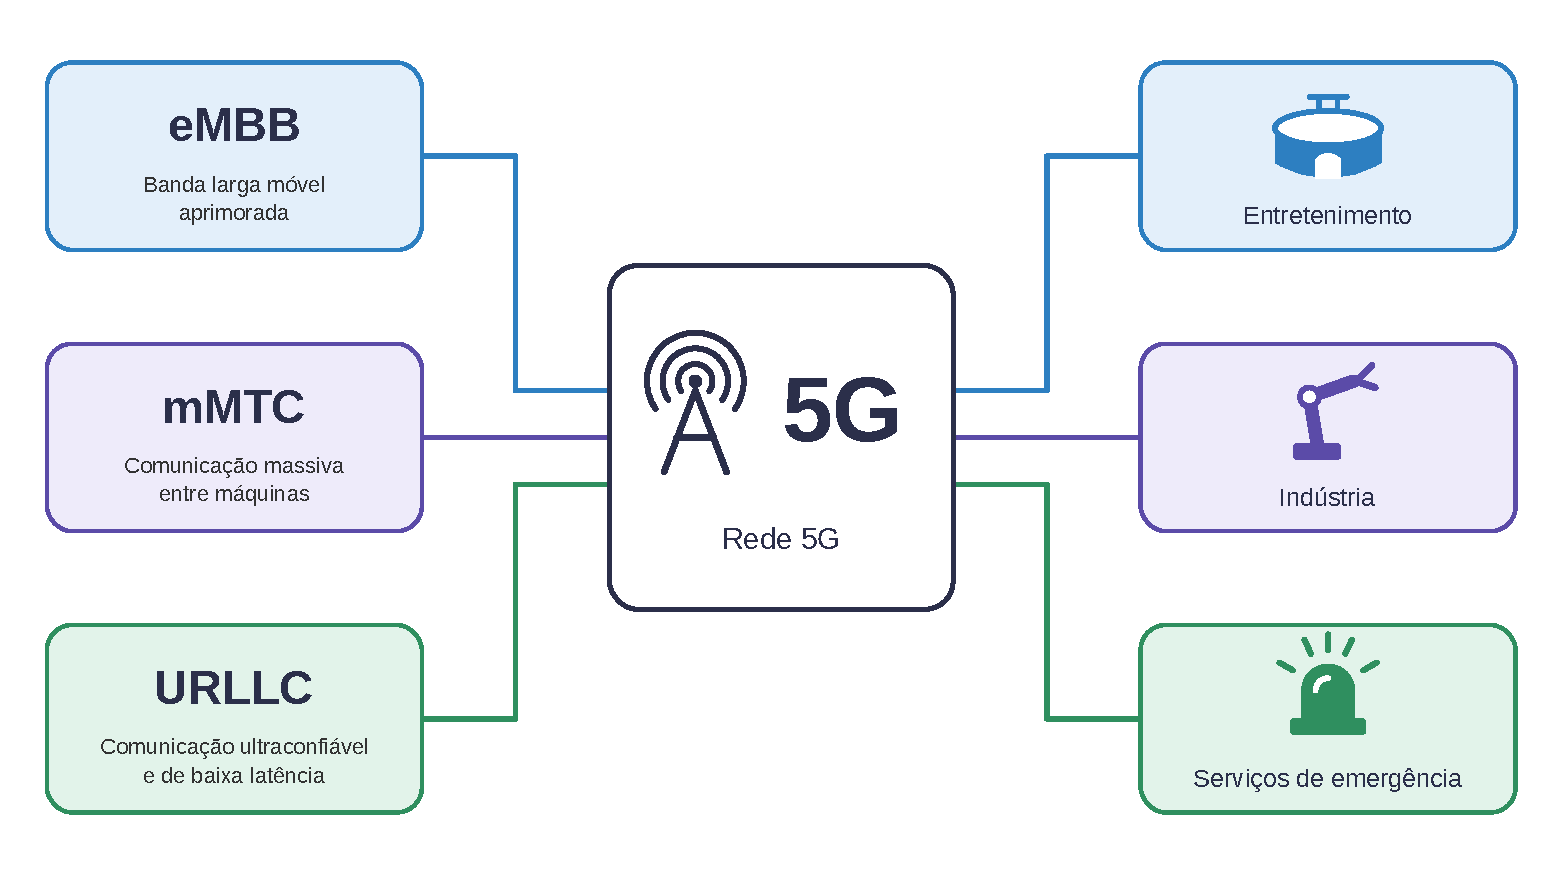
\includegraphics[width=0.6\textwidth]{figuras/fatiamento_5g.pdf}
    \label{fig:fatiamento_5g}
    \fonte{Adaptado de \textcite{inseego2026slicing}.}
\end{figure}

Conforme ilustrado na Figura~\ref{fig:fatiamento_5g}, um desafio crítico na concretização do fatiamento reside no mapeamento consistente entre os identificadores de fatia da camada de serviço (tais como o parâmetro S-NSSAI em redes 5G/6G ou marcações de classe de serviço na borda) e os mecanismos de isolamento na rede de transporte \cite{kotulski20205g, 8436847}. O isolamento entre fatias classifica-se fundamentalmente em dois níveis \cite{kotulski20205g}:
\begin{itemize}
    \item \textbf{Isolamento Lógico:} separação dos planos de controle, endereçamento e políticas de roteamento entre diferentes inquilinos (\textit{tenants}), impedindo vazamento de tráfego ou conflitos de configuração;
    \item \textbf{Isolamento de Desempenho:} garantia de que variações bruscas de carga, rajadas ou congestionamentos originados em uma fatia não degradem as métricas de vazão, latência ou perda de pacotes das demais fatias que compartilham os mesmos enlaces e roteadores físicos \cite{afolabi2018network, kotulski20205g}.
\end{itemize}

% ==============================================================================
\section{Qualidade de Serviço, Escalonamento e Controle de Congestionamento}
\label{sec:qos_escalonamento}

\subsection{Modelos de QoS e Diferenciação de Tráfego}
\label{subsec:modelos_qos}

Para prover isolamento de desempenho em redes de pacotes, duas arquiteturas clássicas foram padronizadas pelo IETF: os Serviços Integrados (\textit{Integrated Services} -- IntServ), baseados na reserva explícita de recursos por fluxo individual mediante sinalização (RSVP), cuja escalabilidade é severamente limitada pela necessidade de manter estados por fluxo em todos os roteadores do núcleo; e os Serviços Diferenciados (\textit{Differentiated Services} -- DiffServ), que agrupam o tráfego em classes agregadas na borda da rede por meio da marcação do campo DSCP (\textit{Differentiated Services Code Point}) no cabeçalho IP \cite{Laki2021, puttaswamy2025pathaware}.

Embora o modelo DiffServ escale adequadamente no núcleo ao eliminar estados por fluxo, sua eficácia depende diretamente das políticas de encaminhamento por salto (\textit{Per-Hop Behaviors} -- PHB) e dos algoritmos de escalonamento configurados nas interfaces de saída de cada comutador \cite{turkovic2021p4qos}. Sem o alinhamento entre a seleção da rota e o tratamento nas filas intermediárias, fluxos marcados com alta prioridade ainda podem sofrer degradação caso sejam encaminhados por enlaces congestionados ou mal dimensionados \cite{wei2026panqosr}.

\subsection{Disciplinas de Enfileiramento e Escalonamento Programável}
\label{subsec:disciplinas_filas}

Nos dispositivos de rede, quando a taxa de chegada de pacotes excede a capacidade instantânea de transmissão de uma interface de saída, os quadros são armazenados em \textit{buffers} e arbitrados por uma disciplina de escalonamento (\textit{packet scheduler}), cujo comportamento determina o atraso de enfileiramento, a variação do atraso (\textit{jitter}, definida pela RFC~3550) e a repartição da largura de banda entre os fluxos:

\begin{itemize}
    \item \textbf{FIFO (\textit{First-In, First-Out}):} disciplina padrão na qual todos os pacotes compartilham uma única fila e são servidos estritamente por ordem de chegada. Embora apresente complexidade computacional mínima, o FIFO não oferece qualquer isolamento: fluxos volumosos de longa duração (\textit{elephant flows}) preenchem o \textit{buffer} (\textit{bufferbloat}) e impõem atrasos elevados e imprevisíveis a fluxos curtos sensíveis à latência (\textit{mice flows}) \cite{santos2024mtspolka}.
    \item \textbf{Prioridade Estrita (\textit{Strict Priority} -- SP):} segrega o tráfego em múltiplas filas hierárquicas e garante que uma fila de menor precedência somente seja atendida quando todas as filas de prioridade superior estiverem completamente vazias. Embora minimize a latência e o \textit{jitter} de aplicações críticas, a prioridade estrita sem controle de admissão ou limitação de taxa pode provocar a inanição (\textit{starvation}) completa dos fluxos de menor prioridade \cite{Elbediwy2025}.
    \item \textbf{\textit{Weighted Deficit Round-Robin} (WDRR):} extensão ponderada do algoritmo \textit{Deficit Round-Robin} (DRR) que permite o compartilhamento justo e proporcional de largura de banda entre múltiplas filas com pacotes de tamanho variável, sem exigir conhecimento prévio do tamanho médio dos quadros \cite{4489385}. A cada ciclo, cada fila ativa recebe um crédito em bytes (\textit{quantum}) proporcional ao peso atribuído à sua classe de serviço; um pacote é transmitido se seu tamanho for inferior ou igual ao déficit acumulado da fila, preservando o saldo remanescente para a rodada seguinte. Além de evitar a inanição, o WDRR possui natureza conservadora de trabalho (\textit{work-conserving}), permitindo que filas ativas aproveitem dinamicamente a largura de banda ociosa de filas vazias \cite{4489385, Elbediwy2025}.
    \item \textbf{Escalonamento Híbrido (SP-WDRR):} combina filas de prioridade estrita no topo da hierarquia --- destinadas a tráfegos de tempo real ou sinalização crítica com taxa estritamente limitada --- com filas escalonadas via WDRR para o tráfego elástico restante, conciliando garantias determinísticas de baixa latência com repartição ponderada de banda.
\end{itemize}

Com o advento dos planos de dados programáveis, pesquisas recentes propuseram abstrações como o PIFO (\textit{Push-In First-Out}) \cite{Sivaraman2016}, o SP-PIFO \cite{Alcoz2020} e gerenciadores de tráfego programáveis baseados em classificações \cite{Elbediwy2024, Elbediwy2025} para superar a rigidez dos escalonadores fixos em comutadores P4 e emuladores como o BMv2. De forma complementar, no \textit{kernel} Linux, o subsistema \textit{Traffic Control} (\texttt{tc}) oferece implementações nativas de disciplinas hierárquicas e sem classes (como \texttt{drr}, \texttt{tbf}, \texttt{netem} e \texttt{bfifo}), permitindo que programas eBPF direcionem pacotes diretamente às filas de saída por meio de metadados do \texttt{sk\_buff} \cite{sharaf2022extended}.

\subsection{Algoritmos de Controle de Congestionamento: CUBIC e BBR}
\label{subsec:controle_congestionamento}

O desempenho observado pelas aplicações em redes fatiadas também sofre influência direta dos algoritmos de controle de congestionamento executados na camada de transporte dos hospedeiros, os quais determinam como os fluxos TCP disputam a capacidade residual das filas:

\begin{itemize}
    \item \textbf{CUBIC (Baseado em Perda):} algoritmo padrão na maioria das distribuições Linux modernas, que ajusta a janela de congestionamento (\textit{cwnd}) segundo uma função cúbica do tempo decorrido desde o último evento de perda de pacotes. Por depender do descarte de pacotes para detectar o congestionamento, o CUBIC tende a preencher continuamente os \textit{buffers} dos roteadores intermediários até provocar perdas, gerando um comportamento oscilatório em dente de serra e elevando o atraso de enfileiramento \cite{Laki2021}.
    \item \textbf{BBR (\textit{Bottleneck Bandwidth and Round-trip propagation time} -- Baseado em Modelo):} em vez de utilizar a perda de pacotes como sinal primário de congestionamento, o BBR estima continuamente duas grandezas fundamentais do caminho: a largura de banda máxima disponível no gargalo (\textit{BtlBw}) e o menor tempo de ida e volta de propagação (\textit{RTprop}). A partir dessas estimativas, o algoritmo regula a cadência de envio (\textit{pacing}) para manter o volume de dados em trânsito próximo ao produto banda-atraso (\textit{Bandwidth-Delay Product} -- BDP), alternando fases periódicas de sondagem de banda e de latência mínima (\textit{ProbeRTT}) a fim de maximizar a vazão sem saturar as filas da rede.
\end{itemize}

% ==============================================================================
\section{Trabalhos Relacionados}
\label{sec:trabalhos_relacionados}

Diversas propostas na literatura investigam a provisão de Qualidade de Serviço, engenharia de tráfego e fatiamento em planos de dados programáveis e redes cientes de caminho. A Tabela~\ref{tab:trabalhos_relacionados} apresenta uma síntese comparativa entre as principais abordagens correlatas e a arquitetura \nome\ proposta nesta dissertação.

\begin{table}[!htb]
    \centering
    \caption{Comparação entre trabalhos relacionados e a arquitetura \nome.}
    \label{tab:trabalhos_relacionados}
    \begin{tabularx}{\textwidth}{Xcccc}
        \toprule
        \textbf{Proposta / Referência} & \textbf{\shortstack{Núcleo sem\\Estado}} & \textbf{\shortstack{Rota Explícita\\na Origem}} & \textbf{\shortstack{Seleção de Fila\\por Salto}} & \textbf{\shortstack{Escalonamento\\Ponderado}} \\
        \midrule
        \textbf{Segment Routing} \cite{rfc8402}        & Parcial\textsuperscript{*} & Sim & Não & Não \\
        \textbf{RDNA} \cite{liberato2018rdna}          & Sim & Sim & Não & Não \\
        \textbf{ProgLab} \cite{froes2020proglab}       & Sim & Sim & Sim & Não \\
        \textbf{PolKA} \cite{dominicini2020}           & Sim & Sim & Não & Não \\
        \textbf{P4QoS / Virtual Queues} \cite{turkovic2021p4qos, harkous2021virtual} & Não & Não & Sim & Sim \\
        \textbf{SP-PIFO / TM Prog.} \cite{Alcoz2020, Elbediwy2025} & Não & Não & Sim & Sim \\
        \textbf{PanQoSR} \cite{wei2026panqosr}         & Parcial\textsuperscript{*} & Sim & Não & Não \\
        \textbf{App-Aware SR} \cite{puttaswamy2025pathaware} & Parcial\textsuperscript{*} & Sim & Indireta\textsuperscript{**} & Sim \\
        \midrule
        \textbf{SPolKA (Este Trabalho)}                & \textbf{Sim} & \textbf{Sim} & \textbf{Sim} & \textbf{Sim} \\
        \bottomrule
    \end{tabularx}
    \fonte{Elaborado pelo autor (2026). \textsuperscript{*}Exige remoção ou atualização de rótulos a cada salto. \textsuperscript{**}Baseada em mapeamento DiffServ/DSCP tradicional.}
\end{table}

As soluções baseadas em escalonamento programável no plano de dados, tais como P4QoS \cite{turkovic2021p4qos}, filas virtuais em P4 \cite{harkous2021virtual}, gerenciamento ativo de filas (\textit{Active Queue Management} -- AQM) em P4 \cite{kundel2018p4, papagianni2019pi2, qiao2022fine}, filas multinível \cite{iqbal2023p4}, SP-PIFO \cite{Alcoz2020} e gerenciadores de tráfego programáveis baseados em classificação \cite{Elbediwy2025}, oferecem controle refinado sobre o atraso e a repartição de banda nas interfaces de saída. Entretanto, essas abordagens concentram-se exclusivamente no comportamento local de enfileiramento dos comutadores, dependendo de tabelas de fluxo e manutenção de estado por classe ou fluxo no núcleo, sem integração nativa com roteamento explícito na origem.

No domínio do roteamento na origem e redes cientes de caminho, propostas como o \textit{Segment Routing} \cite{rfc8402}, o PanQoSR \cite{wei2026panqosr} e o roteamento ciente de aplicação de \textcite{puttaswamy2025pathaware} permitem direcionar fluxos por trajetórias com restrições de QoS. Contudo, o empilhamento de identificadores de segmento exige manipulação de cabeçalhos a cada salto, enquanto o tratamento de filas permanece desacoplado do rótulo de roteamento, dependendo de marcações estáticas como DSCP ou MPLS TC. De modo análogo, o encaminhamento sem estado no núcleo baseado em núcleo sem estado com QoS de \textcite{Laki2021} desacopla atraso e largura de banda, mas não oferece controle explícito de trajetória na origem.

Por fim, entre as arquiteturas baseadas no Sistema Numérico de Resíduos (RNS), a RDNA \cite{liberato2018rdna} e o ProgLab \cite{froes2020proglab} demonstraram a viabilidade de codificar caminhos e rótulos de QoS em identificadores residuais. Entretanto, ambos empregam aritmética modular inteira de precisão arbitrária, cujas operações de divisão inteira não são suportadas nativamente em taxa de linha pelos comutadores programáveis comerciais. Por outro lado, o protocolo \polka\ \cite{dominicini2020} e suas extensões para telemetria \cite{pereira2024mpolkaint}, comprovação de trânsito \cite{borges2024pot} e divisão multicaminho \cite{santos2024mtspolka} superaram a barreira computacional ao migrar para a aritmética polinomial em $GF(2)$ via unidades de CRC, mas restringiram-se à seleção de interfaces físicas de saída sem suporte a filas de serviço.

O protocolo \nome\ preenche exatamente essa lacuna ao estender a aritmética polinomial em $GF(2)$ do \polka\ para codificar, em um único rótulo imutável inserido na borda, tanto a porta de saída quanto a fila de serviço em cada salto, acoplando a decodificação sem estado no núcleo a escalonadores ponderados (WDRR e SP-WDRR) tanto em ambientes P4 quanto no \textit{kernel} Linux via eBPF/XDP.